\chapter{Experimental evaluation}
\label{ch:evaluation}

In this chapter, we present experimental results on the system proposed. Two types of evaluations are present: a first assessment done on the working prototype running on multiple Virtual Machines (VMs) and an evaluation of the performance of the approach, measured using a simulation run on a discrete-event simulator.
In the first case, since it's not possible to emulate a network similar to a real edge network due to the amount of resources needed, we focus on the effectiveness, efficiency and usability of the framework.
While with the discrete-event simulation at hand we can focus on the performance obtained and the resources consumed.
In both scenarios we compare the proposed approach to a typical core-centric approach.



\section{Emulation}
TODO



\section{Simulation}
Using a popular discrete-event simulator written in Python, called SimPy \cite{simpy}, we developed a simulation of our approach. Then we compared our approach with the simulation of a core-centric approach.


\subsection{Components}
To simulate the framework we developed the following abstract components in SimPy:
\begin{itemize}
    \item \inlinecode{Client}: a simplified abstraction of a machine that sends or requests data;
    \item \inlinecode{Transmission}: a simplified abstraction of a virtual link between two machines;
    \item \inlinecode{ProcessingUnit}: a simplified abstraction of a machine that performs a processing job;
\end{itemize}

In the following section we see in the details the behaviour of these abstract components, and their respective realization.


\subsubsection{Client}
There are two realizations of the \inlinecode{Client} abstract component:
\begin{itemize}
    \item \inlinecode{DataProducerClient}: produces a message with a significant amount of data and always sends the message in a deterministic way to a single \inlinecode{ProcessingUnit} (when simulating our edge approach it sends the message to the lowest level of the hierarchy);
    \item \inlinecode{DataReaderClient}: that produces a message with a small amount of data, this message is used to simulate the retrieval of aggregated data. In the edge scenario the level contacted to make the read request can be any level of the hierarchy.
\end{itemize}


\subsubsection{Transmission}
The \inlinecode{Transmission} component allows to simulate the communication between a \inlinecode{Client} and a \inlinecode{ProcessingUnit} or between two \inlinecode{ProcessingUnit} components.
The \inlinecode{Transmission} is initialized with two inputs: the information about the distance between the two machines and a boolean value (\inlinecode{is\_weak\_network}) specifying if the communication passes through only the faster backbone network. The job of the \inlinecode{Transmission} component is converting the two inputs into a single value of latency and simulating this latency.

To compute the latency the \inlinecode{Transmission} component does as follows:

\[ latency = network\_delay +  distance\_delay \]

\[
    network\_delay= 
\begin{cases}
    weak\_network\_delay,    & \text{if } is\_weak\_network\\
    robust\_network\_delay,  & \text{otherwise}
\end{cases}
\]

\[ distance\_delay = \frac{distance}{SPEED\_OF\_SIGNAL} \]

The \inlinecode{network\_delay} is a value representing a constant latency toll that needs to be paid when making the communication, this value depends only on the \inlinecode{is\_weak\_network} boolean. The network which is used by the client (i.e., Wi-Fi, LTE, copper cables) is considered to be weak.

The \inlinecode{distance\_delay} is a value that is proportional to the distance that the signal needs to travel.

The constant \inlinecode{SPEED\_OF\_SIGNAL} is computed in the following way:

\[ SPEED\_OF\_SIGNAL = c \cdot 0.67 \cdot 0.50 \cdot \frac{1}{\sqrt{2}} \]

Where \inlinecode{c} is the speed of light in a vacuum; 0.67 denotes how fast a signal travels through the optical fiber media \cite{optical-fiber-latency}; 0.50 is used to take into consideration the round trip time; \(\frac{1}{\sqrt{2}}\) ($\approx$0.707) is used to take into consideration the fact that cables cannot make a direct path between two points, this offset allows us to put as input the straight line distance between two points.


\subsubsection{ProcessingUnit}
A \inlinecode{ProcessingUnit} component waits for data coming from a \inlinecode{Transmission} component. When new data arrives it is put in an unbounded queue that is used by the cores for starting the processes, so by having \textit{N} cores it means that the \inlinecode{ProcessingUnit} can execute \textit{N} processes in parallel.
When a core is free it takes as input the data from the queue and starts simulating the data processing. The simulation time needed for the data processing is computed as the sum of \inlinecode{start\_delay} and \inlinecode{time\_to\_process}. The value of \inlinecode{start\_delay} is used to simulate a constant delay needed to start the processing and initializing the required resources, while \inlinecode{time\_to\_process} is a value that is computed as:

\[ time\_to\_process = \frac{megabytes\_of\_data}{bandwidth\_capability} \]

Where \inlinecode{megabytes\_of\_data} represents the quantity of data sent in the message and \inlinecode{bandwidth\_capability} represents the Megabytes per unit of time that the core can process. As we will see, a core of an edge device is assumed to be less performing than a core in a big cloud data-center.

The realizations of \inlinecode{ProcessingUnit} are shown below in Figure \ref{fig:processing-unit-realizations}.

\begin{figure}[H]
    \centering
    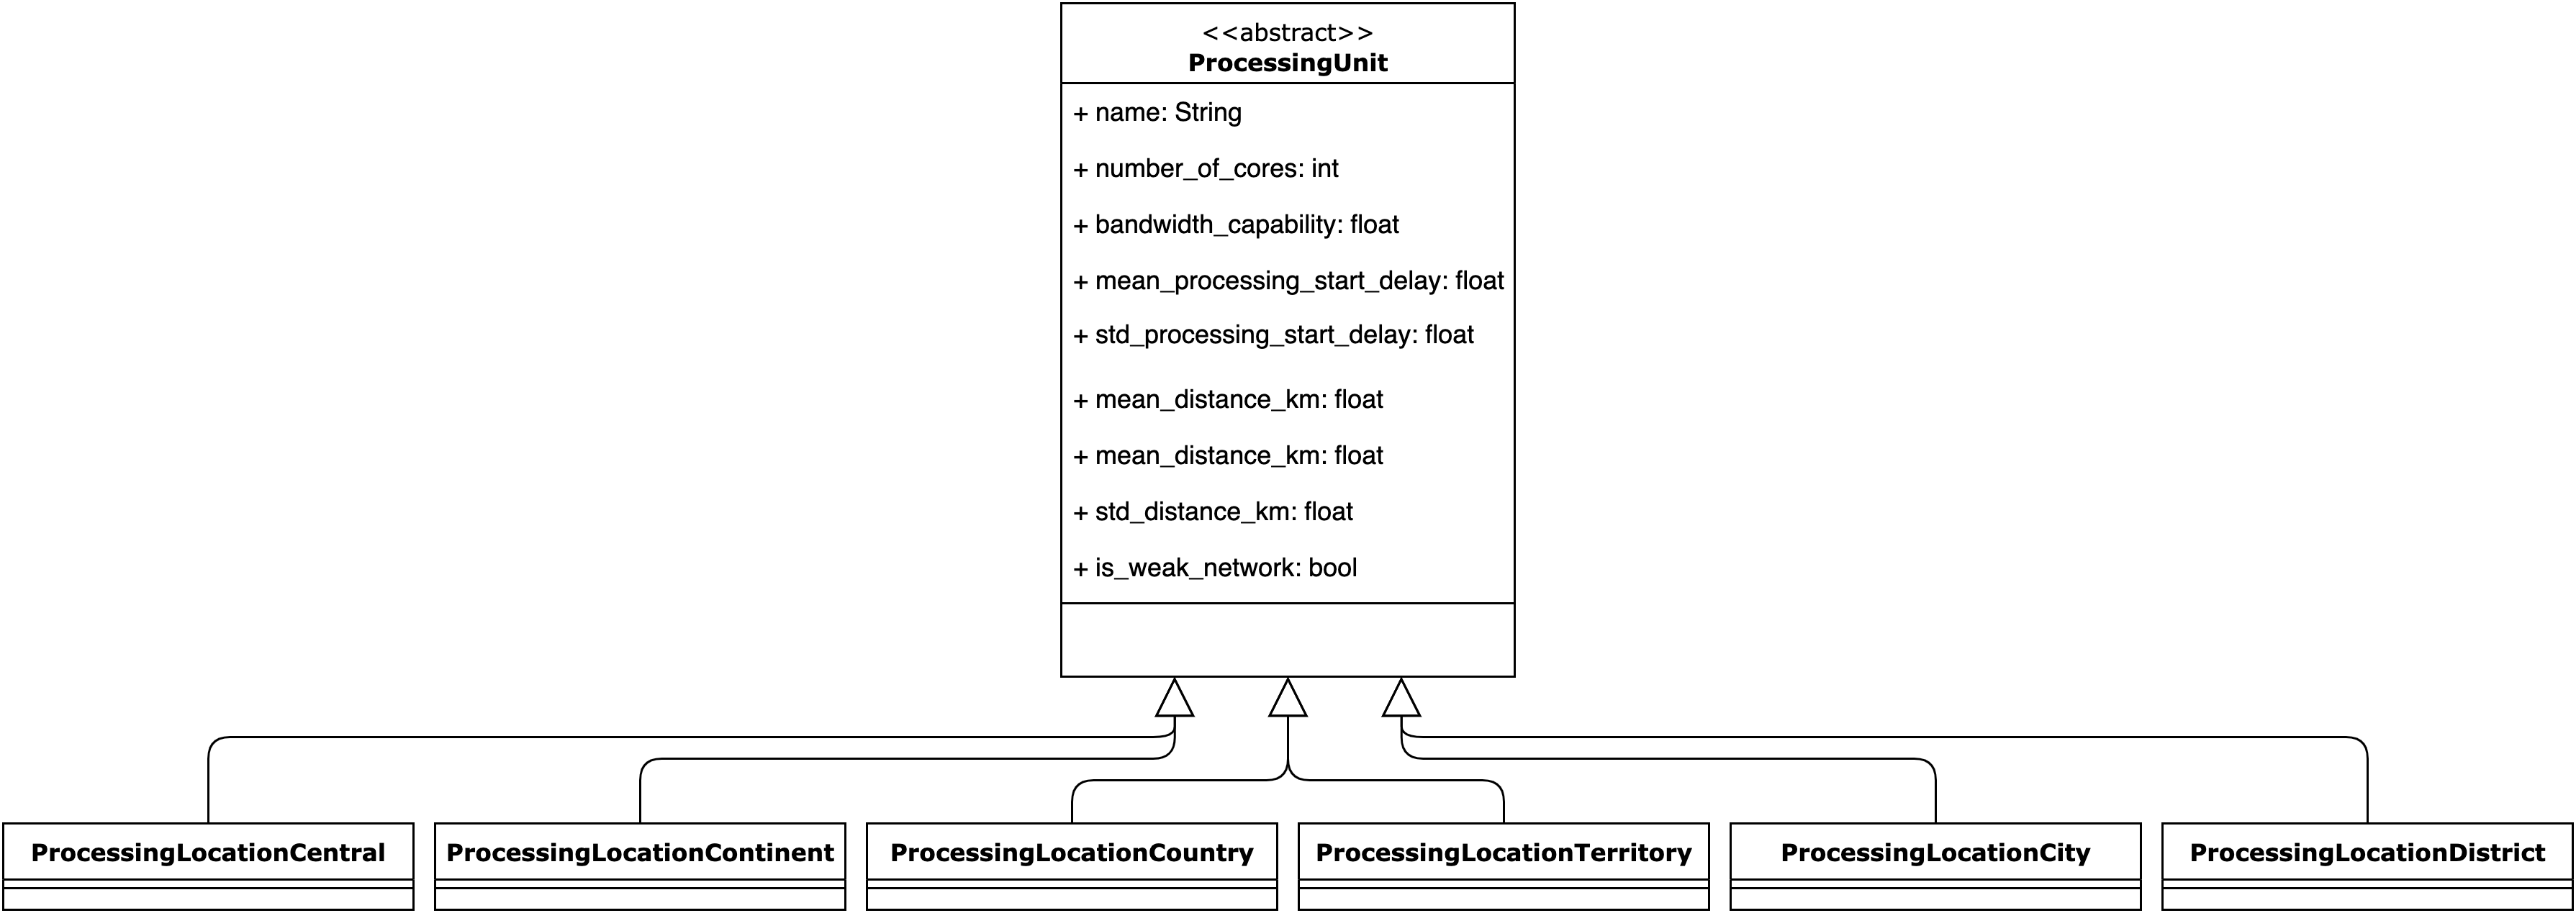
\includegraphics[width=0.99\linewidth]{Figures/Evaluation/processing-unit-realizations.png}
    \caption{Concrete realizations of the ProcessingUnit component.}
    \label{fig:processing-unit-realizations}
\end{figure}


\subsection{Matching the Abstractions to a Use Case}
To better narrow down the abstractions we can see in one of our use cases how these abstractions match a real scenario: in the traffic use case (TODO ref to use case chapter) the \inlinecode{DataProducerClient} represents the camera producing frames of the road. In our edge scenario the camera sends the frame to the lowest level in the hierarchy, which in our example architecture correspond to the "district" level (\inlinecode{ProcessingLocationDistrict}). While in the core-centric scenario the camera sends the frame to the central cloud (\inlinecode{ProcessingLocationCentral}).

The action of sending the frame is simulated using the \inlinecode{Transmission} component. The frame is then processed by applying an image recognition algorithm, an algorithm which is simulated as a data processing by the receiving \inlinecode{ProcessingUnit}.

In the core-centric scenario the output data is ready when finished processing. While in our edge scenario the ouput data is sent to the specified aggregating \inlinecode{ProcessingUnit} which needs to save the data. The communication is again simulated using the \inlinecode{Transmission} component, while the saving of data is simulated as a small processing of data in the aggregating \inlinecode{ProcessingUnit}.

A client can then need to know the traffic in a specific area. This is simulated using the \inlinecode{DataReaderClient} component which can send a read request message, sent using the \inlinecode{Transmission} component and processed by the receiving \inlinecode{ProcessingUnit}.


\subsection{Simulation Setting}
\label{section:simulation_setting}
Since the setting is similar in the various experiments, we present in the tables below the default values of the variables used in the experiments. The actual value will be extracted case by case from a normal distribution truncated to the left at zero. If the standard deviation is zero the value is actually a constant. Unless specified otherwise the values specified here are the ones used in the experiments.

\begin{table}[H]
\centering
\begin{tabular}{|c|c|l|}
\rowcolor{bluepoli!40} % comment this line to remove the color
\hline
\textbf{Variable}       & \textbf{Mean}   & \textbf{Standard deviation}    \\ \hline \hline
Number of clients       & 2000            & 0                              \\ \hline
Time between requests   & 10s             & 3s                             \\ \hline
Message size            & 423KB           & 150KB                          \\ \hline
\end{tabular}
\caption{Default values for variables of DataProducerClient}
\label{tab:default_setting_data_producer}
\end{table}

\begin{table}[H]
\centering
\begin{tabular}{|c|c|l|}
\rowcolor{bluepoli!40} % comment this line to remove the color
\hline
\textbf{Variable}       & \textbf{Mean}   & \textbf{Standard deviation}   \\ \hline \hline
Number of clients       & 2000            & 0                             \\ \hline
Time between requests   & 5s              & 2s                            \\ \hline
Message size            & 10KB            & 1KB                           \\ \hline
\end{tabular}
\caption{Default values for variables of DataReaderClient}
\label{tab:default_setting_data_reader}
\end{table}

\begin{table}[H]
\centering
\begin{tabular}{|c|c|l|}
\rowcolor{bluepoli!40} % comment this line to remove the color
\hline
\textbf{Variable}      & \textbf{Mean}   & \textbf{Standard deviation}   \\ \hline \hline
Weak network delay     & 12ms            & 8ms                           \\ \hline
Robust network delay   & 3ms             & 1ms                           \\ \hline
\end{tabular}
\caption{Default values for variables of Transmission}
\label{tab:default_setting_transmission}
\end{table}

\begin{table}[H]
\centering
\begin{tabular}{|c|c|l|}
\rowcolor{bluepoli!40} % comment this line to remove the color
\hline
\textbf{Variable}               & \textbf{Mean}   & \textbf{Standard deviation}   \\ \hline \hline
Number of districts             & 1000            & 0                             \\ \hline
Distance client-district        & 20km            & 8km                           \\ \hline
Number of cores per district    & 2               & 0                             \\ \hline
Processing bandwidth per core   & 10MB/s          & 0                             \\ \hline
Processing start delay          & 5ms             & 2ms                           \\ \hline
\end{tabular}
\caption{Default values for variables of ProcessingLocationDistrict}
\label{tab:default_setting_district}
\end{table}

\begin{table}[H]
\centering
\begin{tabular}{|c|c|l|}
\rowcolor{bluepoli!40} % comment this line to remove the color
\hline
\textbf{Variable}               & \textbf{Mean}   & \textbf{Standard deviation}   \\ \hline \hline
Number of cities                & 400             & 0                             \\ \hline
Distance client-city            & 60km            & 15km                          \\ \hline
Distance district-city          & 50km            & 15km                          \\ \hline
Number of cores per city        & 2               & 0                             \\ \hline
Processing bandwidth per core   & 10MB/s          & 0                             \\ \hline
Processing start delay          & 5ms             & 2ms                           \\ \hline
\end{tabular}
\caption{Default values for variables of ProcessingLocationCity}
\label{tab:default_setting_city}
\end{table}

\begin{table}[H]
\centering
\begin{tabular}{|c|c|l|}
\rowcolor{bluepoli!40} % comment this line to remove the color
\hline
\textbf{Variable}               & \textbf{Mean}   & \textbf{Standard deviation}   \\ \hline \hline
Number of territories           & 200             & 0                             \\ \hline
Distance client-territory       & 300km           & 100km                         \\ \hline
Distance district-territory     & 290km           & 100km                         \\ \hline
Number of cores per district    & 4               & 0                             \\ \hline
Processing bandwidth per core   & 15MB/s          & 0                             \\ \hline
Processing start delay          & 4ms             & 1ms                           \\ \hline
\end{tabular}
\caption{Default values for variables of ProcessingLocationTerritory}
\label{tab:default_setting_territory}
\end{table}

\begin{table}[H]
\centering
\begin{tabular}{|c|c|l|}
\rowcolor{bluepoli!40} % comment this line to remove the color
\hline
\textbf{Variable}               & \textbf{Mean}   & \textbf{Standard deviation}   \\ \hline \hline
Number of countries             & 80              & 0                             \\ \hline
Distance client-country         & 700km           & 300km                         \\ \hline
Distance district-country       & 690km           & 300km                         \\ \hline
Number of cores per country     & 4               & 0                             \\ \hline
Processing bandwidth per core   & 15MB/s          & 0                             \\ \hline
Processing start delay          & 4ms             & 1ms                           \\ \hline
\end{tabular}
\caption{Default values for variables of ProcessingLocationCountry}
\label{tab:default_setting_country}
\end{table}

\begin{table}[H]
\centering
\begin{tabular}{|c|c|l|}
\rowcolor{bluepoli!40} % comment this line to remove the color
\hline
\textbf{Variable}               & \textbf{Mean}   & \textbf{Standard deviation}   \\ \hline \hline
Number of continents            & 7               & 0                             \\ \hline
Distance client-continent       & 1500km          & 500km                         \\ \hline
Distance district-continent     & 1490km          & 500km                         \\ \hline
Number of cores per continent   & 1000            & 0                             \\ \hline
Processing bandwidth per core   & 20MB/s          & 0                             \\ \hline
Processing start delay          & 4ms             & 1ms                           \\ \hline
\end{tabular}
\caption{Default values for variables of ProcessingLocationContinent}
\label{tab:default_setting_continent}
\end{table}

\begin{table}[H]
\centering
\begin{tabular}{|c|c|l|}
\rowcolor{bluepoli!40} % comment this line to remove the color
\hline
\textbf{Variable}           & \textbf{Mean}   & \textbf{Standard deviation}   \\ \hline \hline
Distance client-central     & 5000km          & 2000km                        \\ \hline
Distance district-central   & 4990km          & 2000km                        \\ \hline
Number of cores             & 1000            & 0                             \\ \hline
Processing bandwidth        & 20MB/s          & 0                             \\ \hline
Processing start delay      & 4ms             & 1ms                           \\ \hline
\end{tabular}
\caption{Default values for variables of ProcessingLocationCentral}
\label{tab:default_setting_central}
\end{table}


\subsection{Results}
In each experiment we ran our SimPy simulation and let thousands of clients connect to the thousands of cloudlets and data centers, we collected data about latencies, distances and traffic and now we show in this section the results.
By having many variables extracted from the truncated normal distributions, we are effectively running random experiments where it makes sense to show a confidence interval calculated on the list of samples obtained. But collecting numerous samples is easy in a simulation, in fact we obtained in all the experiments a really tight 95\% confidence interval that cannot even be seen on the plot.


\subsubsection{Write by level}
In this experiment we suppose that the developer wants a single geographical aggregation, this means that we are simulating as if we were using our framework with the \inlinecode{saveAlsoInIntermediateLevels} set to \inlinecode{false}.
The clients send their data to the bottom level of the hierarchy (\inlinecode{ProcessingLocationDistrict} in case of the edge approach, \inlinecode{ProcessingLocationCentral} in case of the cloud approach). The data is then processed and, in the case of the edge approach, forwarded to the \inlinecode{referringArea} that aggregates the data.

\begin{figure}[H]
    \centering
    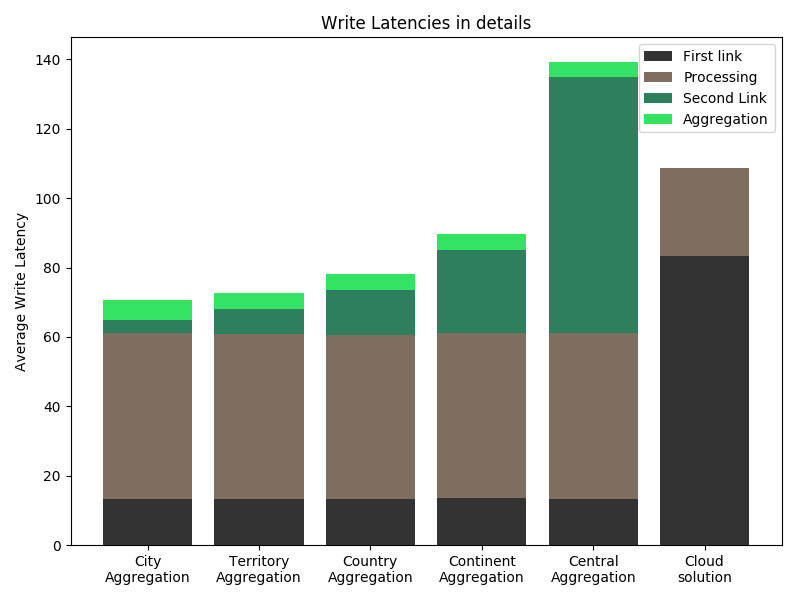
\includegraphics[width=0.86\linewidth]{Figures/Evaluation/write-by-latency2.png}
    \caption{Details on the average write latency compared between various aggregation in the edge setup and compared to the cloud setup.}
    \label{fig:write-by-latency2}
\end{figure}

In Figure \ref{fig:write-by-latency2} we can see the average write latency for each setup. For the edge approach we show the result of five different setups with five different levels of aggregation (city, territory, country, continent, central).
This average write latency comes from four different operations:
\begin{itemize}
    \item First link latency: latency of the communication between the client and the receiving machine.
    \item Processing latency: latency that considers the wait time for a core to be free and the processing time for the data sent by the client. We can see in the plot that the processing time of the cloud solution is close to half of the processing time in the edge setups, this is due the fact that the core bandwidth of a core in \inlinecode{ProcessingLocationCentral} is supposed to be double the core bandwidth of a core in \inlinecode{ProcessingLocationDistrict}.
    \item Second link latency: latency of the communication between the receiving  \inlinecode{ProcessingUnit} and the aggregating \inlinecode{ProcessingUnit}. This latency is only present in the setups using the edge approach.
    \item Aggregation latency: time required by the aggregating \inlinecode{ProcessingUnit} to save the data received from the \inlinecode{ProcessingLocationDistrict}. This time is the sum of the wait time for a core to be free and the time to save the processed data.
\end{itemize}

This result shows that with the edge approach using any aggregation level we have a smaller average latency than the cloud solution thanks to a much smaller travel distance needed to reach the aggregating \inlinecode{ProcessingUnit}. The only exception is the central aggregation of the edge approach, which is expected since it has the same travel distance of the cloud solution, but by doing the processing on the lower level of the hierarchy we have a smaller processing power.

Using this same experiment we now analyze the huge improvements our edge approach gives to the traffic in the network.

\begin{figure}[H]
    \centering
    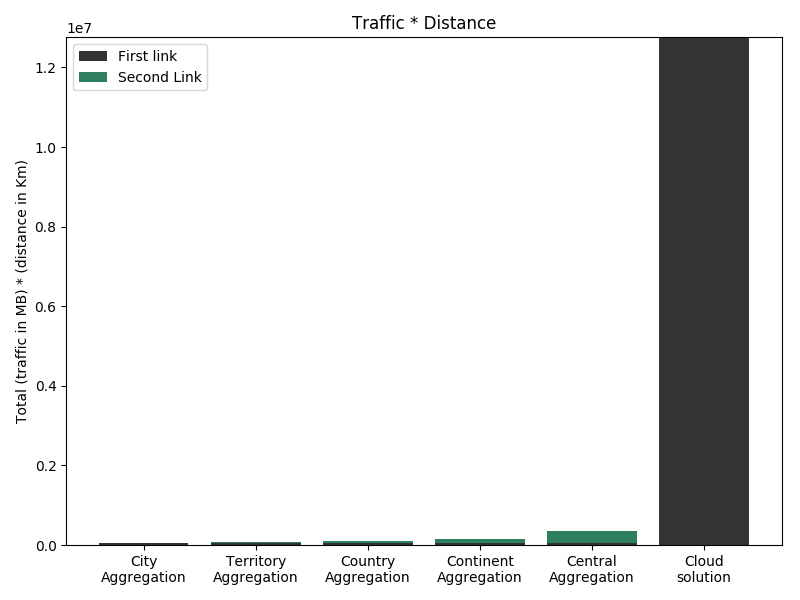
\includegraphics[width=0.86\linewidth]{Figures/Evaluation/write-by-traffic1.png}
    \caption{Traffic per distance generated in the network.}
    \label{fig:write-by-traffic1}
\end{figure}

In Figure \ref{fig:write-by-traffic1} we show the total traffic in megabytes multiplied by the distance travelled. This visualization is used to show that the cloud solution clogs the entire network, instead by processing the data near the client we obtain a huge saving in terms of bandwidth used in the network.

\begin{figure}[H]
    \centering
    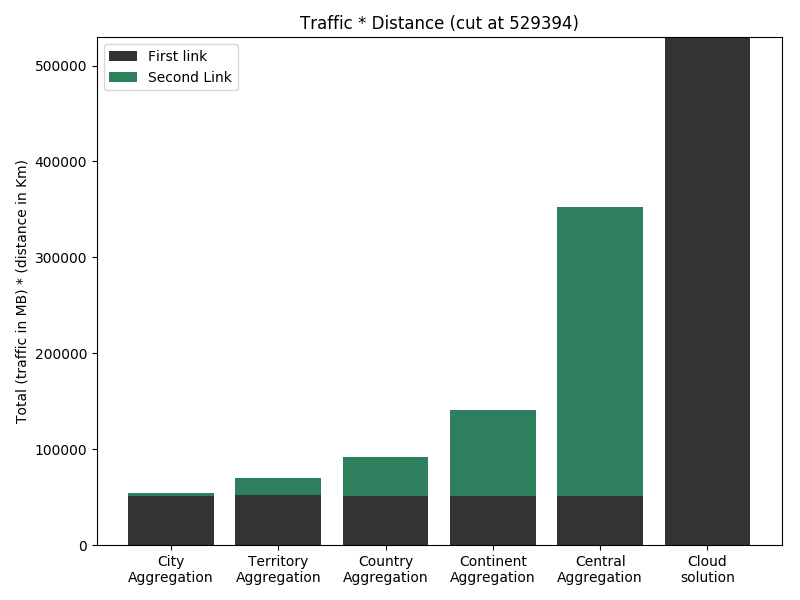
\includegraphics[width=0.86\linewidth]{Figures/Evaluation/write-by-traffic2.png}
    \caption{Traffic per distance generated in the network (cut at a lower traffic*distance value).}
    \label{fig:write-by-traffic2}
\end{figure}

In Figure \ref{fig:write-by-traffic2} we zoom on the values of the setups of the edge approach by cutting the plot at a lower traffic*distance value. We can see how the traffic*distance values in the first link for the edge approach are very much similar since in all five setups we have the same communication between the \inlinecode{DataProducerClient} and the \inlinecode{ProcessingLocationDistrict}. While for the second link we find an increase in the traffic*distance due to the fact that the distance increases between the \inlinecode{ProcessingLocationDistrict} and the aggregating \inlinecode{ProcessingUnit}.


\subsubsection{Write all levels}
In this experiment, for the edge approach, we suppose that the developer uses the boolean \inlinecode{saveAlsoInIntermediateLevels} set to \inlinecode{true} and sets the \inlinecode{referringAreaType} in our framework to the highest level of the hierarchy (central). Meaning that all writes made at the receiving  \inlinecode{ProcessingLocationDistrict} are forwarded to the upper levels. This setup is compared to the cloud setup in which data are sent to a central data center that can aggregate them by location.

Writes to upper levels happen in parallel, so we expect to have an average latency similar to the latency of the edge setup with central aggregation of the previous experiment. This is in fact what we obtain as can be seen in Figure \ref{fig:write-all-latency}. In terms of latency we are clearly in a case of disadvantage here since as it has been seen in the previous experiment that by doing a central aggregation, like the cloud approach does, we are not exploiting our edge approach to the max.

\begin{figure}[H]
    \centering
    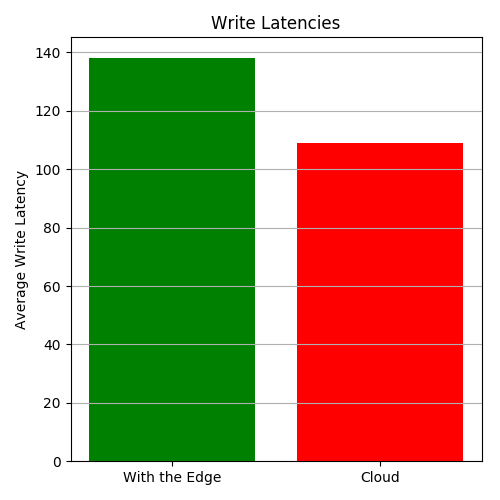
\includegraphics[width=0.75\linewidth]{Figures/Evaluation/write-all-latency.png}
    \caption{Average write latency of the single edge setup compared to the cloud setup.}
    \label{fig:write-all-latency}
\end{figure}

Many more messages are sent in parallel to the various aggregating \inlinecode{ProcessingUnit} so we expect the traffic*distance in the network to increase compared to the previous experiment. This is in fact true as can be seen in Figure \ref{fig:write-all-traffic1}, but still the cloud setup clogs the network 2000\% more than the edge setup.

\begin{figure}[H]
    \centering
    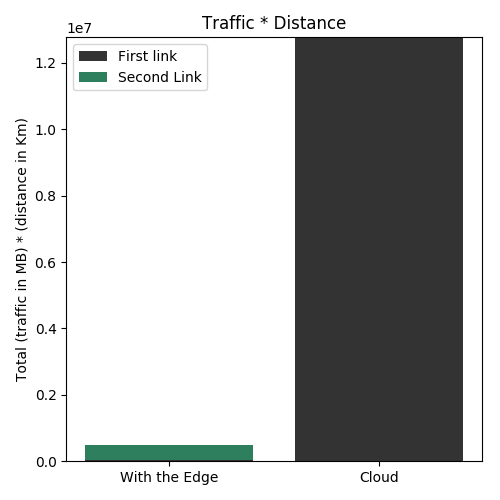
\includegraphics[width=0.75\linewidth]{Figures/Evaluation/write-all-traffic1.png}
    \caption{Traffic per distance generated in the network.}
    \label{fig:write-all-traffic1}
\end{figure}

We saw in this experiment that even in a disadvantage situation where our approach is used to aggregate the data in a central manner, which is not the intended use case, the increase in write latency is less than 27\%, but the improvement in terms of traffic sent in the network is tremendous.


\subsubsection{Write all levels, with cores performance as parameter}
As in the previous experiment we are working in a scenario where the developer imposes writes on all levels in the edge approach.

In our simulation we represented the performance of the cores as a processing bandwidth, so we specified how much megabytes a core can process in a second. In the previous experiments we used the default values reported in Section \ref{section:simulation_setting}, so we arbitrarily assumed that the \inlinecode{ProcessingLocationDistrict} and \inlinecode{ProcessingLocationCity} have 50\% of the performance of \inlinecode{ProcessingLocationCentral}. We now analyze the behaviour of the latency while slowly changing this percentage to show that the increase in write latency is not substantial.

\begin{figure}[H]
    \centering
    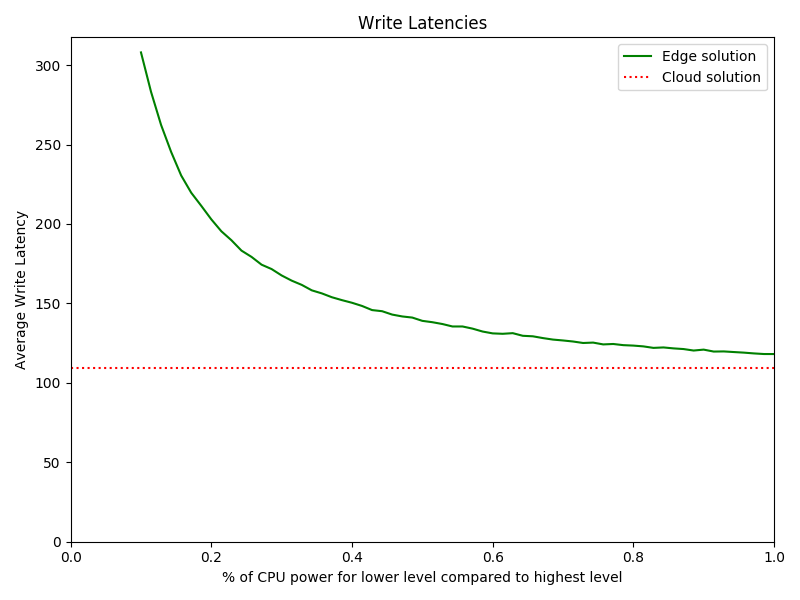
\includegraphics[width=0.86\linewidth]{Figures/Evaluation/write-all-cpu-latency.png}
    \caption{Average write latency of the edge solution as a function of the cores performance of lower levels}
    \label{fig:/write-all-cpu-latency}
\end{figure}

In Figure \ref{fig:/write-all-cpu-latency} it is shown the changing write latency of the edge solution due to the changing performance of the \inlinecode{ProcessingUnits} cores, compared to the constant latency of the cloud solution.

Note that the value 0.1 on the x-axis means that the performance of the core at the edge is 0.1 times (10\%) the performance of the core of cloud solution.

From 1.0 to 0.40 we have an almost linear increase, which is not substantial. Then down from 0.40 the cores can't keep up with the requests and start to put them in queue, creating an exponential increase in the latency.

So this experiment shows the following:
\begin{itemize}
    \item By having a lower performance in the \inlinecode{ProcessingUnits} at the edge the processing latency increase linearly, making the write latency also increase linearly;
    \item By having a lower performance in the \inlinecode{ProcessingUnits} at the edge it becomes easier to reach a limit where the cores can't keep up with the requests, creating an exponential increase in the write latency.
\end{itemize}


\subsubsection{Write all levels, with number of clients as parameter}
In this experiment we are again working in the scenario where the developer imposes writes on all levels while using the edge approach. But now we want to simulate, in this extreme setup, how our framework behaves when the number of clients rises without modifying other parameters.
We start from 1000 clients, rising up to 350'000 clients.

\begin{figure}[H]
    \centering
    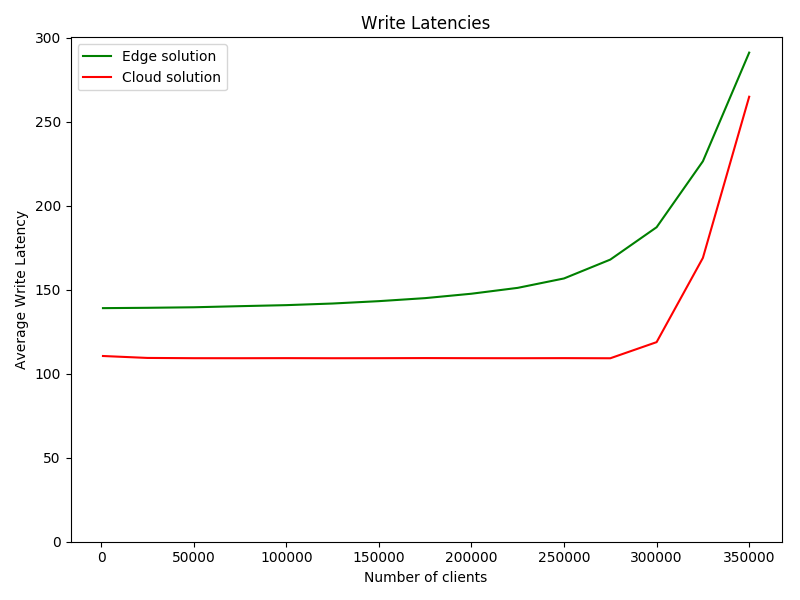
\includegraphics[width=0.86\linewidth]{Figures/Evaluation/write-all-clients-latency.png}
    \caption{Average write latency as a function of the number of clients}
    \label{fig:/write-all-clients-latency}
\end{figure}

As expected we see in Figure \ref{fig:/write-all-clients-latency} that, when the number of clients becomes too much to handle, both the cores at the edge and the cores in the cloud are overwhelmed and can't keep up with the requests causing the queues to grow indefinitely and consequently making the average latency grow.

We can also notice how the number of cores affects the latency: in the edge approach by having a low number of cores it's easier to be unlucky and having a momentary spike where the \inlinecode{ProcessingLocationDistrict} can't keep up with the requests, causing new requests to be queued for a short time. Basically by increasing the number of clients it become more probable to have a random spike in the requests, that a single \inlinecode{ProcessingLocationDistrict} cannot handle immediately since equipped with only 2 cores. This phenomenon causes a continuous increase in the average latency for the edge solution.
Instead in the cloud solution, to start to queue requests we have to first fill the 1000 cores, and for that to happen it needs many more clients.

It's important also to consider that in our simulation we are not modelling the access to the database: in a cloud scenario in which writes happen to a single instance of the database it can easily become a bottleneck if not replicated and handed correctly.

But again the improvements relative to the traffic generated in the network are immense. In Figure \ref{fig:/write-all-clients-traffic} we show the total traffic*distance as a function of the number of clients. Both the edge solution and cloud solution have a linear increase, but the coefficient of the increase in the cloud solution is evidently bigger than the one of the edge solution.

\begin{figure}[H]
    \centering
    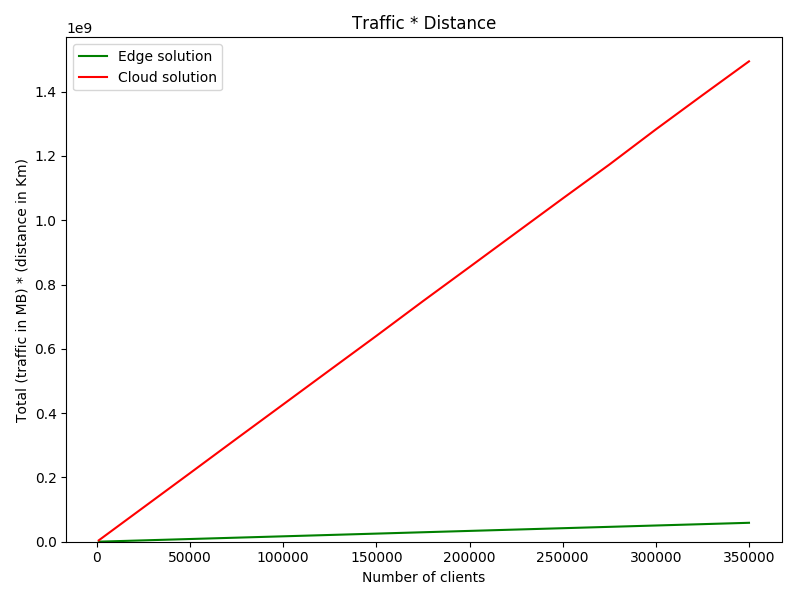
\includegraphics[width=0.86\linewidth]{Figures/Evaluation/write-all-clients-traffic.png}
    \caption{Total traffic*distance as a function of the number of clients}
    \label{fig:/write-all-clients-traffic}
\end{figure}

In this experiment we showed that our framework can keep up effectively with heavy load, with only minor random congestions at the lower levels of the hierarchy. But still provide immensely benefits in term of traffic through the network.


\subsubsection{Read by level}
We now start with a new type of experiment, focusing on the reads and not on the writes. We will immediately see the benefit on the latency since by having a geographical aggregation we can avoid to travel huge distances.
In practice in this experiment we have different setups in which every \inlinecode{DataReaderClients} in the setup communicates to a certain level of the hierarchy of the edge solution. While in the cloud solution they can only communicate to the central cloud.
In the figures reported below we can see, for each level of aggregation, the average latency and the average distance traveled, compared to the cloud solution.

\begin{figure}[H]
\begin{minipage}{0.49\textwidth}
\centering
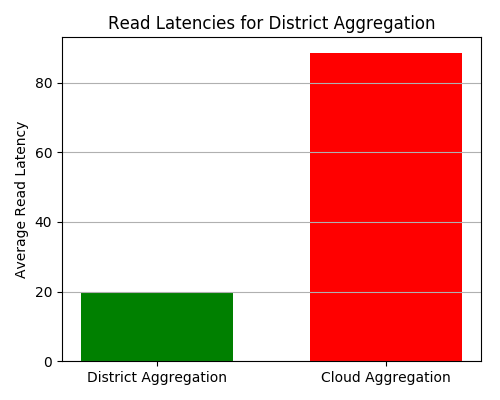
\includegraphics[width=1\linewidth]{Figures/Evaluation/read-by-latency-District-Aggregation.png}
\end{minipage}
\hfill
\begin{minipage}{0.49\textwidth}
\centering
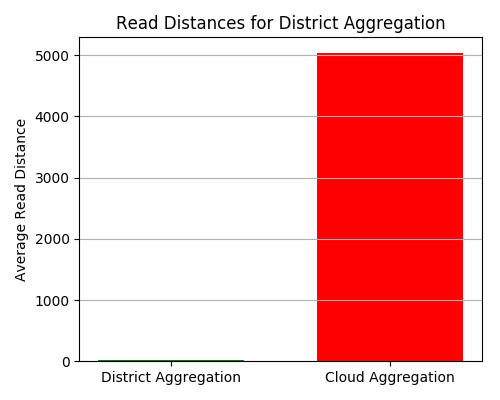
\includegraphics[width=1\linewidth]{Figures/Evaluation/read-by-distance-District-Aggregation.png}
\end{minipage}
\label{fig:read-by-district}
\caption{Average latency and average distance traveled for the district aggregation compared to a central aggregation}
\end{figure}

\begin{figure}[H]
\begin{minipage}{0.49\textwidth}
\centering
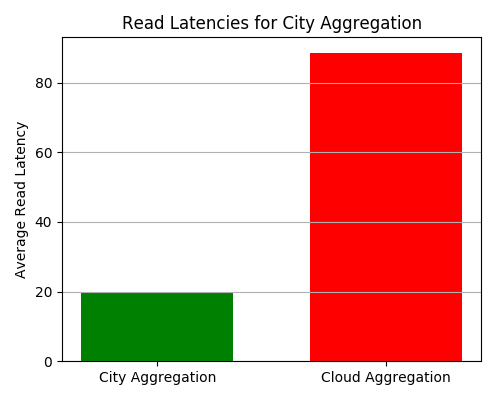
\includegraphics[width=1\linewidth]{Figures/Evaluation/read-by-latency-City-Aggregation.png}
\end{minipage}
\hfill
\begin{minipage}{0.49\textwidth}
\centering
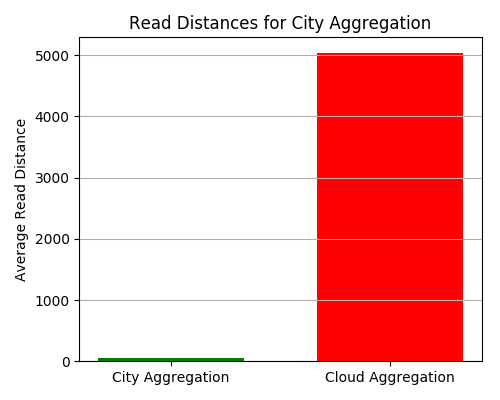
\includegraphics[width=1\linewidth]{Figures/Evaluation/read-by-distance-City-Aggregation.png}
\end{minipage}
\label{fig:read-by-city}
\caption{Average latency and average distance traveled for the city aggregation compared to a central aggregation}
\end{figure}

\begin{figure}[H]
\begin{minipage}{0.49\textwidth}
\centering
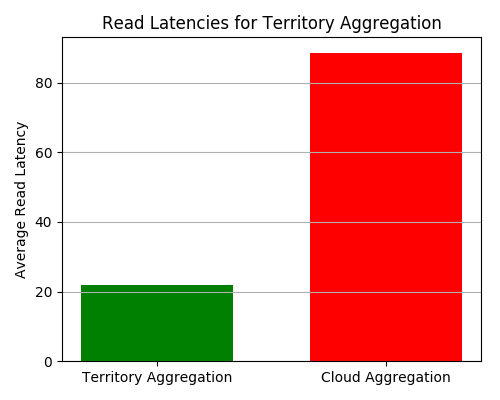
\includegraphics[width=1\linewidth]{Figures/Evaluation/read-by-latency-Territory-Aggregation.png}
\end{minipage}
\hfill
\begin{minipage}{0.49\textwidth}
\centering
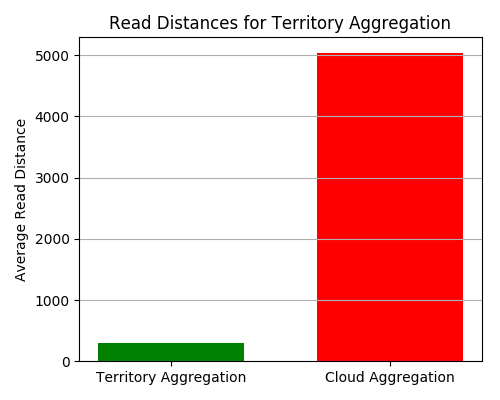
\includegraphics[width=1\linewidth]{Figures/Evaluation/read-by-distance-Territory-Aggregation.png}
\end{minipage}
\label{fig:read-by-territory}
\caption{Average latency and average distance traveled for the territory aggregation compared to a central aggregation}
\end{figure}

\begin{figure}[H]
\begin{minipage}{0.49\textwidth}
\centering
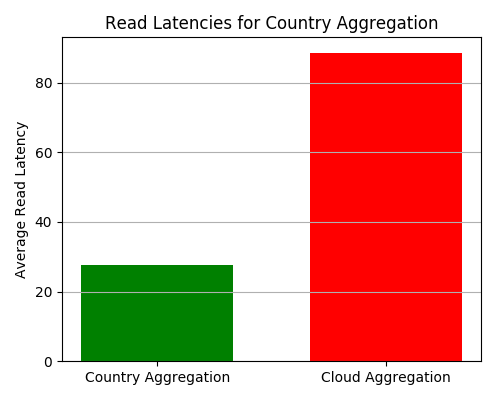
\includegraphics[width=1\linewidth]{Figures/Evaluation/read-by-latency-Country-Aggregation.png}
\end{minipage}
\hfill
\begin{minipage}{0.49\textwidth}
\centering
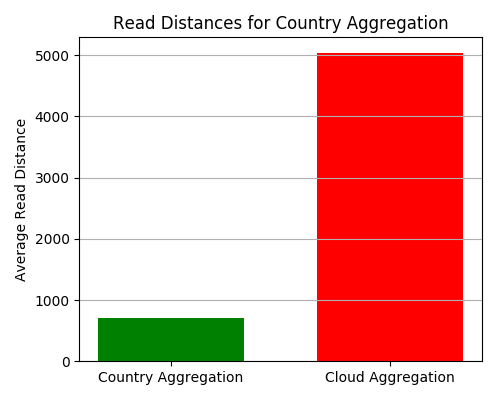
\includegraphics[width=1\linewidth]{Figures/Evaluation/read-by-distance-Country-Aggregation.png}
\end{minipage}
\label{fig:read-by-country}
\caption{Average latency and average distance traveled for the country aggregation compared to a central aggregation}
\end{figure}

\begin{figure}[H]
\begin{minipage}{0.49\textwidth}
\centering
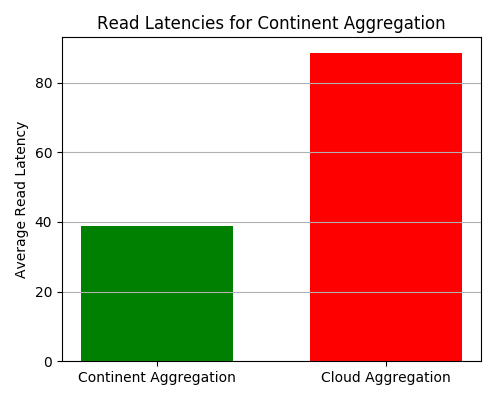
\includegraphics[width=1\linewidth]{Figures/Evaluation/read-by-latency-Continent-Aggregation.png}
\end{minipage}
\hfill
\begin{minipage}{0.49\textwidth}
\centering
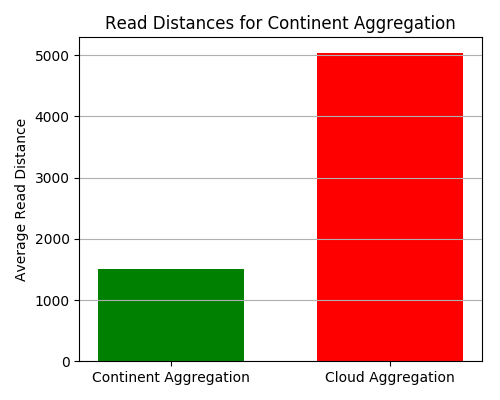
\includegraphics[width=1\linewidth]{Figures/Evaluation/read-by-distance-Continent-Aggregation.png}
\end{minipage}
\label{fig:read-by-continent}
\caption{Average latency and average distance traveled for the continent aggregation compared to a central aggregation}
\end{figure}

If we go up in the hierarchy to perform the aggregation we become more distant to the reading client, creating a bigger latency on average.

We can see also how the average latency is proportional to the average distance: when the distance increases, so does the latency due to the bigger travel distance.

If we compare the best scenario, in which the aggregation is performed at the lowest level, to the cloud solution we see that the cloud solution creates a latency 350\% bigger than the district (19.5 ms compared to 88.5 ms). 


\subsubsection{Read all levels}
This time we allow clients to perform the reads on every level, this means that to have the data available the writes must have happen with the \inlinecode{saveAlsoInIntermediateLevels} boolean set to \inlinecode{true}.
In the 51 setups that we ran we increased the probability of making a read on an upper level of the hierarchy. The first setup performs all the read requests at the district level, in the intermediate setup the clients perform the read requests with almost an equal probability to all levels, while the last setup performs all the read requests to the single central level.

\begin{figure}[H]
    \centering
    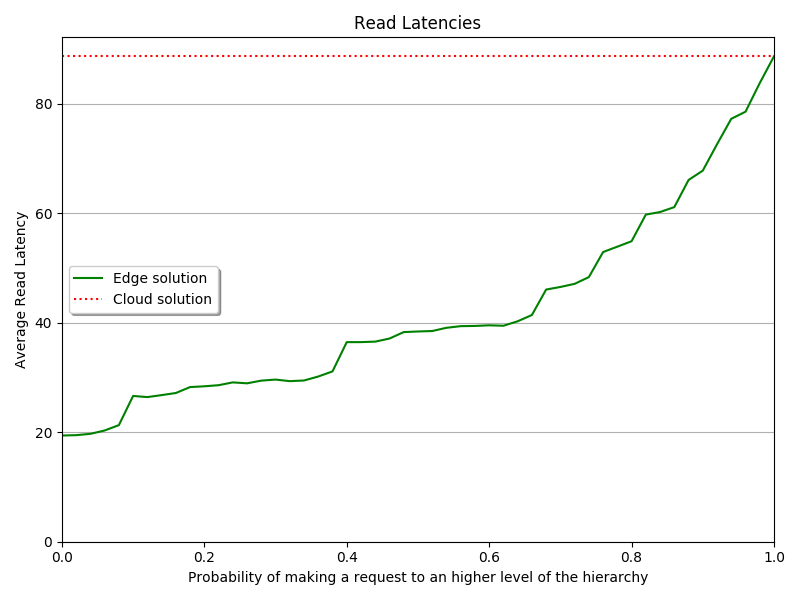
\includegraphics[width=0.86\linewidth]{Figures/Evaluation/read-all-latency.png}
    \caption{Average read latency as a function of the probability of making the read request to an higher level}
    \label{fig:/read-all-latency}
\end{figure}

\begin{figure}[H]
    \centering
    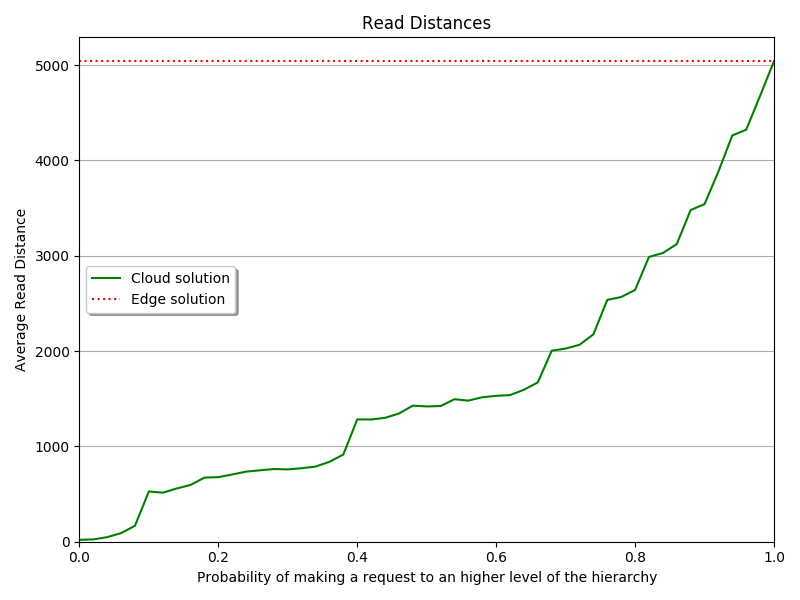
\includegraphics[width=0.86\linewidth]{Figures/Evaluation/read-all-distance.png}
     \caption{Average distance traveled for the request as a function of the probability of making the read request to an higher level}
    \label{fig:/read-all-distance}
\end{figure}

As expected we see a monotonic increase in the latency and a strict correlation between the average distance traveled and the average latency.

\subsubsection{Read district level, with cores performance as parameter}
In this experiment clients make read requests to the lowest level of the hierarchy, the district level, and we study the latency as a function of the cores performance of this level.
We arbitrarily assumed that the \inlinecode{ProcessingLocationDistrict} has 50\% of the performance of \inlinecode{ProcessingLocationCentral}, but now we slowly change this percentage to analyze the behaviour of the latency.

\begin{figure}[H]
    \centering
    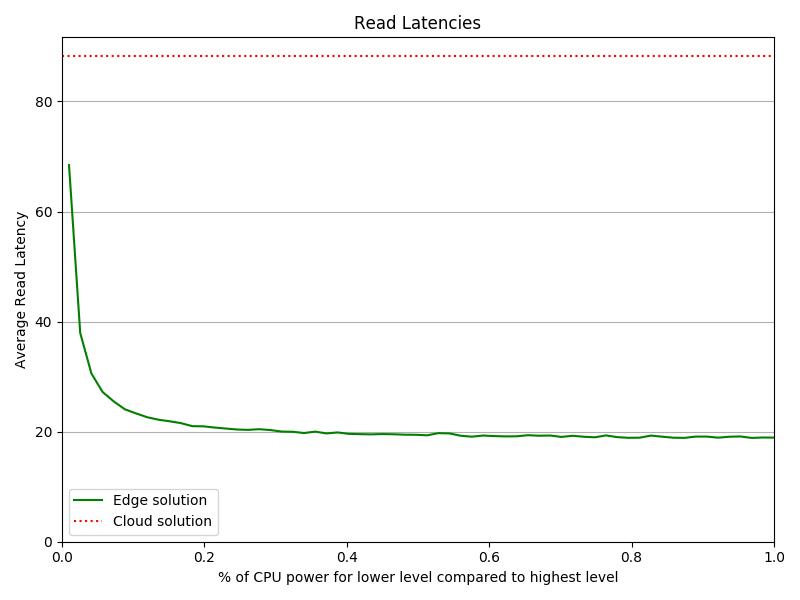
\includegraphics[width=0.86\linewidth]{Figures/Evaluation/read-district-cpu-latency.png}
    \caption{Average read latency of the edge solution as a function of the cores performance of lower levels}
    \label{fig:/read-district-cpu-latency}
\end{figure}

As can be seen in Figure \ref{fig:/read-district-cpu-latency}, the effects of slower cores start to affect the latency only when reaching very low percentages i.e., 10\%, and still even at 1\% of the performance the latency is smaller than the one of the cloud solution. This is because a read request is a fast operation and is not a processing intensive task, so the cores can manage the load comfortably.

\subsubsection{Read district level, with number of clients as parameter}
As a last experiment we see how the framework performs in the simulations with a varying number of clients (and consequently a varying load).
Similarly here read requests are made to the lowest level of the hierarchy, the district level.

\begin{figure}[H]
    \centering
    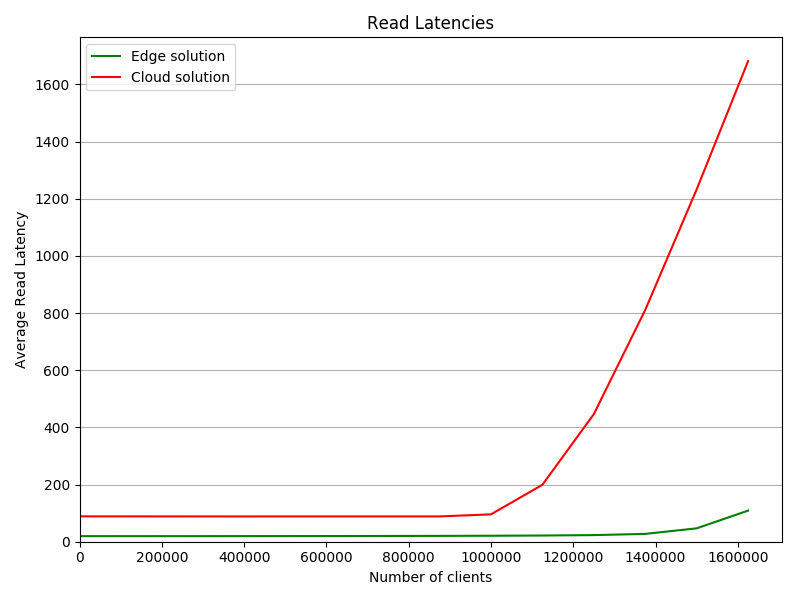
\includegraphics[width=0.86\linewidth]{Figures/Evaluation/read-district-clients-latency.png}
    \caption{Average read latency of the edge solution as a function of the number of clients}
    \label{fig:/read-district-clients-latency}
\end{figure}

The read operation is a fast operation that does not require heavy processing, this allows both the cloud solution and the edge solution to fulfill a million of requests in a small amount of time before starting to not keep up with the load.

\subsection{Summing Up}
Thanks to the simulation and by performing the various experiments we showed that by using our framework we get immense benefits in terms of reduced traffic in the network while allowing faster reads when the data aggregation needed is not central.
In a case where a central aggregation is still needed we showed that the write requests suffer an increase in latency, but the increase is not substantial.

We also noticed how our edge solution can be affected by random spikes in the requests due to the small number of cores and resources in the lowest level of the hierarchy, so there is a clear room for improvements on this matter, but still the increase in latency is not drastic.

